\lecture{VPN ({\em Virtual Private Network})}

\lecturetitle{\course}{\insertlecture}

\frame{\maketitle}

\begin{frame}{}
  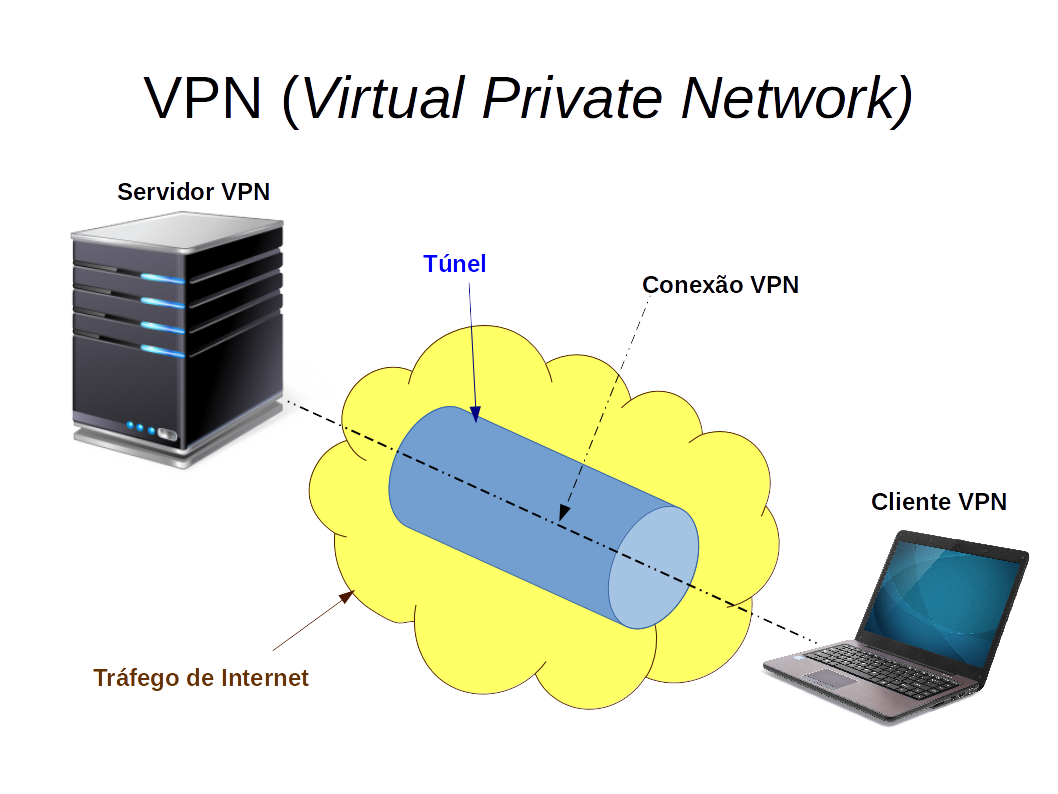
\includegraphics[scale=.39]{img/vpn.png}
\end{frame}

\begin{frame}{\insertlecture}\small

  \begin{itemize}[<+->]\setbeamercovered{transparent}
  \item É a extensão de uma rede privativa que passa por
    compartilhamentos ou rede pública como a Internet.
  \item Para emular um link ponto a ponto, os dados são encapsulados,
    ou empacotados, com um cabeçalho que fornece informações de
    roteamento para atravessar a rede pública.
  \item Os dados são indecifráveis na rede pública, pois necessitam
    das chaves criptográficas.
  \item A parte da conexão em que os dados estão encapsulados é
    conhecida como túnel.
  \item A parte da conexão em que os dados estão criptografados é
    conhecida como rede virtual privativa (VPN–Virtual Private
    Network).
  \end{itemize}
  
\end{frame}

\begin{frame}{Tunelamento}

  \begin{itemize}[<+->]\setbeamercovered{transparent}
  \item {\bf Tunelamento} é o método de usar a infraestrutura de inter-rede
    para transferir os dados de uma rede para outra.
  \item Ao invés de enviar o quadro como foi produzido na origem, o
    {\bf protocolo de tunelamento} encapsula o quadro em um cabeçalho
    adicional.
\item O caminho lógico dos pacotes entre as redes é chamado de {\bf túnel}.
  \end{itemize}
 
\end{frame}

\begin{frame}{Exemplo de Protocolo de Tunelamento}
  \begin{itemize}
  \item {\bf\em Point-to-Point Tunneling Protocol} (PPTP): o protocolo de
    tunelamento ponto-a-ponto encapsula quadros PPP (protocolo
    ponto-a-ponto) em datagramas IP para transmissão em redes como a
    Internet.

    \bigskip
    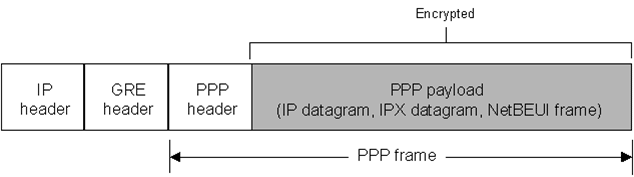
\includegraphics[scale=.45]{img/pptp.png}

  \end{itemize}

\end{frame}

\begin{frame}{Outros Protocolos de Tunelamento}
  \begin{itemize}[<+->]\setbeamercovered{transparent}
  \item {\em Internet Protocol Security} (IPSec) Tunnel Mode:
    protocolo de internet seguro em modo túnel.
  \item {\em Layer Two Tunneling Protocol} (L2TP): protocolo de
    tunelamento na camada dois.
  \end{itemize}
\end{frame}

\begin{frame}{Requisitos Básicos da VPN}

  \begin{description}[<+->]\setbeamercovered{transparent}
  \item[Autenticação do usuário:] o acesso à VPN é restrito a usuários identificados.
  \item[Gerenciamento de endereços:] um endereço privativo deve ser atribuído para o cliente.
  \item[Criptografia de dados:] os dados não podem ser lidos na rede pública.
  \item[Gerenciamento de chaves:] devem ser geradas e atualizadas
    chaves criptográficas no cliente e servidor.
  \item[Suporte a vários protocolos:] a VPN deve gerenciar os
    protocolos também utilizados na rede pública, tais como, {\em
      Internet Protocol} (IP), {\em Internet Packet Exchange} (IPX),
    {\em Domain Name Service} (DNS), dentre outros.
  \end{description}
  
\end{frame}

\begin{frame}{Auditoria da VPN}
  
  \begin{itemize}[<+->]\setbeamercovered{transparent}
  \item O administrador da VPN deve rastrear o número de conexões,
    atividades irregulares, condições de erro e falha em equipamentos.
  \item O tempo de conexão do usuário também deve ser possível de ser
    auditados para fins de cobrança.
  \end{itemize}
\end{frame}

\begin{frame}{Benefícios da VPN}

  \begin{itemize}[<+->]\setbeamercovered{transparent}
  \item Comunicação segura de dados institucionais.
  \item Uso dos benefícios da rede institucional, tais como licenças
    de software, assinatura de revistas científicas e jornais, acesso
    à recursos fornecidos pela instituição, em qualquer lugar com
    acesso à rede pública.
  \end{itemize}
  
\end{frame}